\documentclass[conference]{IEEEtran}
\usepackage{cite}
\usepackage{amsmath,amssymb}
\usepackage{graphicx}
\usepackage{booktabs}
\usepackage{array}
\usepackage{tabularx}
\usepackage{url}
\usepackage[hidelinks]{hyperref}

% Many figures: let floats fill the top of a page.
\renewcommand{\dbltopfraction}{0.9}
\renewcommand{\dblfloatpagefraction}{0.6}
\renewcommand{\topfraction}{0.9}
\renewcommand{\floatpagefraction}{0.7}
\setcounter{dbltopnumber}{3}
\setcounter{topnumber}{3}

\begin{document}

\title{AstroFixxer: An Offline Smartphone Push-To Guide\\with On-Device Plate Solving for Small Telescopes}

% Author details: replace the bracketed fields before submission.
\author{\IEEEauthorblockN{[Author name]}
\IEEEauthorblockA{{[Department], [Institution]}\\
{[City], [Country]}\\
kushmodi13@gmail.com}}

\maketitle

\begin{abstract}
Beginners with manual Dobsonian and small alt-azimuth telescopes often cannot find faint objects, because the mount gives no readout of where the tube points. Commercial answers add encoders or a camera dock, and the free phone apps that replace them rely on the phone's compass and gyroscope, which drift and are disturbed by a metal tube. This paper reviews the free and commercial tools in this space and describes AstroFixxer, an open-source Android application that guides a telescope from a phone strapped to it. AstroFixxer extends the AstroHopper web application with a Stellarium-derived offline catalogue of 93,997 deep-sky objects, 8,913 stars and the IAU constellation boundaries, a star-alignment step, and a plate solver written in pure Kotlin that runs on the phone against 579,984 stars to magnitude 10.5 from Gaia DR3 and Hipparcos. The previous sidereal-time formula left pointing errors of up to 801 arcseconds against the astropy reference; the corrected precession model reduces the worst of 66 reference cases to 28 arcseconds. On synthetic star fields the solver solved all 29 test images, including 1-degree eyepiece fields to within 0.5 arcseconds, and refused all 28 negative cases, among them random-star fields. The application has not yet been validated with a real telescope, and the paper states which parts remain to be tested in the field.
\end{abstract}

\begin{IEEEkeywords}
amateur astronomy, push-to navigation, smartphone sensors, plate solving, star identification, offline mobile application
\end{IEEEkeywords}

\section{Introduction}

A 150 mm or 200 mm Dobsonian telescope shows hundreds of galaxies and clusters, yet many first-time owners see only the Moon and the planets. The mount is two bearings and a tube. It has no setting circles, the finder shows a small patch of sky, and most deep-sky objects are too faint to see in it. Observers traditionally reach them by star hopping from a bright star with a paper chart, a skill that takes many nights to learn.

Three kinds of tools address this. Digital setting circles fit encoders to both axes and report the tube's altitude and azimuth to a handset or a planetarium app such as SkySafari~\cite{skysafari}. Camera-based finders photograph the sky and identify the star pattern: Celestron's StarSense Explorer does this with the phone's own camera looking into a mirror dock~\cite{starsense}, and the open-source PiFinder uses a Raspberry Pi camera~\cite{pifinder}. The third group uses a phone strapped to the tube as the sensor. AstroHopper~\cite{astrohopper} and SkEye~\cite{skeye} read the phone's gyroscope, gravity sensor and compass, and ask the observer to point at one known star so that the app can remove the compass offset. This last approach needs no extra hardware, but the compass is unreliable next to a steel tube and the gyroscope drifts within minutes, so the observer has to realign often.

AstroFixxer started as a web port of AstroHopper and is now a native Android application. It keeps the free, sensor-based design and adds the pieces that the review in Section~\ref{sec:related} finds missing from the free tools: a large offline catalogue, an explicit and correctable alignment step, and camera plate solving that runs on the phone without a network connection or a dock.

The contributions described in this paper are:
\begin{itemize}
\item a review of free and commercial push-to tools and plate solvers, compared by the hardware they need, how they determine pointing, and whether they work offline (Section~\ref{sec:related}, Table~\ref{tab:compare});
\item an offline data pipeline that converts Stellarium's catalogues into compact Android assets, including 579,984 Gaia- and Hipparcos-based stars for plate solving (Section~\ref{sec:data});
\item a corrected coordinate model whose worst error against astropy falls from 801 to 28 arcseconds over 66 reference cases (Section~\ref{sec:core});
\item a pure-Kotlin plate solver with a statistical acceptance test, evaluated on synthetic wide-field and eyepiece images (Section~\ref{sec:solver}).
\end{itemize}

Section~\ref{sec:related} reviews related software and algorithms. Section~\ref{sec:system} describes what AstroFixxer implements, Section~\ref{sec:design} shows its design in UML diagrams, and Section~\ref{sec:review} compares it with the reviewed tools and lists what has not yet been tested. Section~\ref{sec:conclusion} concludes.

\section{Related Work}
\label{sec:related}

\subsection{Phone-sensor push-to applications}

AstroHopper by Artyom Beilis is a free progressive web application released under the GPLv3~\cite{astrohopper}. Its author describes it as digital setting circles implemented in a smartphone. The phone is attached to the tube with its top edge pointing along the optical axis. The observer centres a known star, presses Align, waits about three seconds for the sensors to settle, and then moves the telescope until the displayed altitude and azimuth differences reach zero. The app needs a gyroscope and a gravity sensor; the compass is optional, and a manual azimuth mode covers phones without one. It works offline once cached and offers watch lists, a night mode and user-defined objects. AstroFixxer is a derivative of this code and keeps its licence.

SkEye is an Android planetarium with a push-to mode~\cite{skeye}. In its ``indirect mode'' the observer points the telescope at a known object and tells the app what it is; the app stores the angular offset between the phone and the tube and then follows the phone's compass, accelerometer and gyroscope. SkEye comes in a free Basic and a paid Pro version.

Both apps share the same weak point. The alignment offset is correct only while the sensors stay calibrated, and a magnetometer next to a steel tube or a metal mount is easily disturbed. Neither app can check its own pointing against the sky.

Sky Map (formerly Google Sky Map) is an open-source Android sky viewer that uses the same sensors to show the part of the sky the phone points at~\cite{skymap}. It shipped on the first Android phones, was open-sourced in 2012, and the current rewrite is GPLv3. It is not designed to be mounted on a telescope, but it is the best-known free example of sensor-driven sky display on Android.

\subsection{Camera-based pointing}

Celestron's StarSense Explorer holds the phone in a dock above a small mirror, so the rear camera sees the sky the telescope points at~\cite{starsense}. The companion app plate-solves the camera image with a ``lost in space'' algorithm to find where the telescope points. Celestron says this was the first app to use plate solving for this purpose and that the technology is patented. The app works only with the StarSense Explorer telescopes that include the dock.

PiFinder is open-source hardware and software built around a Raspberry Pi, the Raspberry Pi HQ camera and a small display~\cite{pifinder}. It solves the sky image up to 20 times a second and uses an accelerometer between exposures to update the chart and the push-to directions. It needs no alignment and no encoders, and it offers a catalogue of about 150,000 objects. Its plate solving uses the Cedar Detect and Cedar Solve libraries, which descend from tetra3.

These two systems show what a camera adds: the pointing is measured, not inferred from drifting sensors. Both need dedicated hardware: a dock tied to one telescope range, or a separate computer and camera.

\subsection{Planetarium software with telescope control}

Stellarium is a GPL desktop planetarium used both by amateurs and in cultural-astronomy research~\cite{zotti2021}. It includes a telescope control plugin for motorised mounts, and its catalogues, sky cultures and star files are published with the source. AstroFixxer takes all of its offline sky data from Stellarium. SkySafari is a commercial planetarium for phones and tablets~\cite{skysafari}. It connects to digital setting circle encoders and GoTo mounts, draws the telescope's field of view on the chart, and relies on the encoders for pointing.

\subsection{Plate-solving and star-identification algorithms}

Astrometry.net solves an image with no prior knowledge of where it points or of its scale~\cite{lang2010}. It detects sources, forms geometric hashes of groups of four or five stars, looks them up in pre-built index files, and accepts a hypothesis only if it passes a Bayesian decision test against the null hypothesis that the matches are chance. Covering a wide range of image scales needs large index files, which suits a desktop or a server better than a phone.

Tetra identifies stars from a single database access by storing star patterns in a directly addressed hash table~\cite{tetra2017}. It was designed for spacecraft star trackers, where the field of view is fixed and known, and it won the student competition at the 2017 Small Satellite Conference. Its open-source Python descendant tetra3 underlies the libraries used by PiFinder.

ASTAP is a free, open-source stacking program with a fast local plate solver~\cite{astap}. It solves FITS, raw and common image formats on desktop systems and the Raspberry Pi against downloadable star databases, which are offered at several star densities.

Marbel, Ben-Moshe and Yozevitch showed that a star tracker can run on a commercial smartphone and recover the phone's global orientation from its own camera~\cite{marbel2020}. Their target was the orientation of drones and nano-satellites, not telescope pointing, but the work shows that phone cameras detect enough stars for pattern matching.

\subsection{Summary}

Table~\ref{tab:compare} compares the tools. The free phone apps need no hardware but cannot verify their pointing. The camera systems measure pointing but need a dock or a separate computer. The solvers are general tools for desktops, servers or spacecraft, not for a phone at the eyepiece. No free tool in this review combines sensor push-to, camera plate solving on the phone itself, and offline operation. That gap is the one AstroFixxer targets.

\begin{table*}[t]
\centering
\caption{Push-to tools and plate solvers reviewed in Section~\ref{sec:related}}
\label{tab:compare}
\small
\setlength{\tabcolsep}{4pt}
\begin{tabularx}{\textwidth}{@{}l l X l l l@{}}
\toprule
Tool & Platform & Pointing from & Extra hardware & Offline & Source \\
\midrule
AstroHopper~\cite{astrohopper} & Web app (PWA) & Phone sensors, one-star alignment & None & Yes, once cached & GPLv3 \\
SkEye~\cite{skeye} & Android & Phone sensors, object offset & None & Yes & Not published \\
Sky Map~\cite{skymap} & Android & Phone sensors (sky viewer only) & None & Yes & Apache 2.0 / GPLv3 \\
StarSense Explorer~\cite{starsense} & iOS, Android & Phone camera, plate solving & Dock and mirror & Yes & Proprietary, patented \\
PiFinder~\cite{pifinder} & Raspberry Pi & Camera plate solving + accelerometer & Pi, camera, display & Yes & Open source \\
SkySafari~\cite{skysafari} & iOS, Android & Encoders or GoTo mount & Encoders or mount & Yes & Proprietary \\
Stellarium~\cite{zotti2021} & Desktop & Mount control plugin & Motorised mount & Yes & GPL \\
Astrometry.net~\cite{lang2010} & Server, desktop & Blind plate solving & Camera & With local index & Open source \\
ASTAP~\cite{astap} & Desktop, Pi & Plate solving & Camera & Yes & Open source \\
\midrule
AstroFixxer (this work) & Android & Phone sensors, star alignment, on-phone plate solving & None & Yes & GPLv3 \\
\bottomrule
\end{tabularx}
\end{table*}

\section{What AstroFixxer Implements}
\label{sec:system}

\subsection{Origin, licence and scope}

AstroFixxer began as a web application derived from AstroHopper~\cite{astrohopper, astrofixxerweb}. Because AstroHopper is GPLv3, the Android port is GPLv3 as well, and its source is public~\cite{astrofixxerandroid}. The Android version keeps AstroHopper's pointing mathematics and adds an offline catalogue, events, a voice assistant and plate solving. It targets Android 8.0 (API level 26) and later.

\subsection{Architecture}

The app is written in Kotlin with Jetpack Compose. It is a single Gradle module with three layers. The astronomy layer (\texttt{astro/}) holds coordinates, catalogues, events, satellite passes and the plate solver, and it has no Android imports, so it runs under plain JVM unit tests. The interface layer (\texttt{ui/}) holds the screen state and the Compose screens; it also has no Android imports, which lets the same code run in a Compose Desktop test harness. Only \texttt{MainActivity} touches Android: sensors, location, speech, preferences and asset loading. The project deliberately avoids a dependency-injection framework, a database and a networking library, since everything the app needs ships in its assets.

\subsection{Offline data}
\label{sec:data}

A Python importer converts Stellarium's data files into the app's assets at build time. The main catalogue holds 93,997 deep-sky objects from Stellarium's catalogue and 8,913 stars from the HYG v3 database~\cite{hyg} with their B$-$V colour indices. It also holds the modern and Indian sky cultures and 781 IAU constellation boundary edges. The boundaries are published for the 1875 equinox, so the importer precesses them to J2000 with the IAU 1976 model~\cite{lieske1977}; the result agrees with astropy~\cite{astropy2022} to 0.37 arcseconds. Comet and asteroid orbital elements and meteor shower data also come from Stellarium, and eclipses come from NASA's published tables.

For plate solving, the importer decodes Stellarium's binary star catalogues, which are built from Gaia DR3~\cite{gaia2023} and Hipparcos~\cite{perryman1997}. It propagates each star from the catalogue epoch to J2000 using its proper motion and keeps 579,984 stars brighter than magnitude 10.5. Each star is stored in 5 bytes, sorted into declination bands and right-ascension cells so that a cone around a pointing can be read without scanning the file. The asset is 2.94 MB. Cross-matched against HYG, the 4,969 stars brighter than magnitude 6 have a median position difference of 0.046 arcseconds.

\subsection{Coordinate model}
\label{sec:core}

Planet positions come from VSOP87~\cite{bretagnon1988} with light time, aberration, precession and a truncated IAU 2000B nutation series, ported from the web application. Satellite passes use SGP4~\cite{vallado2006}.

The web code converted catalogue positions to the local horizon with the Earth rotation angle applied to J2000 coordinates and no precession. Because the Earth rotation angle omits the accumulated precession in right ascension that Greenwich sidereal time contains, this formula happens to cancel most of the precession in right ascension. The part that does not cancel, the change in declination, grows by about 20 arcseconds a year. We measured it against astropy for 12 bright stars on 4 dates and at 3 sites (New Delhi, Sydney and Troms\o), which gives 66 cases above 5 degrees altitude. The worst error was 801 arcseconds.

The corrected model applies each term once. A J2000 unit vector $\mathbf{r}_0$ is rotated to the mean equator of date with the IAU 1976 angles~\cite{lieske1977},
\begin{equation}
\mathbf{r} = R_3(-z)\,R_2(\theta)\,R_3(-\zeta)\,\mathbf{r}_0 ,
\end{equation}
and the hour angle is taken from Greenwich mean sidereal time, $h = \mathrm{GMST} + \lambda - \alpha$, where $\lambda$ is the observer's east longitude and $\alpha$ the right ascension of date. The inverse transformation, used to report where the telescope points, applies the transpose. Nutation (up to 17 arcseconds) and annual aberration (up to 20 arcseconds) are left out on purpose, since the narrowest eyepiece field in use is at least 15 arcminutes across. The worst of the 66 cases is now 28 arcseconds, and the unit tests fail if either correction is applied twice. The precession matrix is cached per time step, because the sky view converts thousands of stars in each frame.

\subsection{Alignment and guidance}

The phone's rotation-vector sensor gives the orientation of the phone, from which the app derives the direction of the telescope axis. The observer centres a bright star in the eyepiece and selects it. The app then computes a rotation that moves its predicted pointing onto the star, in azimuth first and then in altitude, following AstroHopper~\cite{astrohopper}. For a chosen target the app shows the remaining altitude and azimuth, or right ascension and declination for an equatorial mount, together with a bullseye that fills when the target lies inside the eyepiece's true field. The true field is computed from the eyepiece's apparent field and the focal lengths of the eyepiece and the telescope.

At the time of writing, a revised alignment flow is being implemented. It asks for the telescope type, mount and phone placement on first launch. The observer drags the map until the chosen star sits under a fixed centre marker and then confirms. A second star can be added to check and refine the alignment. Section~\ref{sec:review} lists what of this has been tested.

\subsection{On-device plate solver}
\label{sec:solver}

The solver is about 1,200 lines of Kotlin with no native code. It first estimates the image background on a coarse grid and the noise from the median absolute deviation. It then marks pixels about five standard deviations above the background and groups them into connected blobs. Each star position is a flux-weighted centroid, and its elongation comes from second moments. Single hot pixels and saturated regions are discarded. The image is rejected as too bright, trailed or nearly empty before any matching is tried, and the user is told which case applies.

The pixel scale is known within a range from the telescope and eyepiece settings or from the phone camera's focal length. The solver therefore matches triangles of the brightest detected stars against catalogue triangles using real angular side lengths. The magnitude limit is chosen so that the catalogue offers about one to three times as many stars as were detected. Each candidate match gives a similarity transform with a possible mirror flip in a gnomonic projection. The solver projects all catalogue stars in the field, counts detections that land within the centroid tolerance, and refines the fit by least squares.

A wrong answer would send the observer to the wrong part of the sky, so acceptance is strict. A solution needs at least six matched stars spread over at least a quarter of the frame, and a scale inside the hinted range. It also needs a false-alarm probability below $10^{-6}$ after multiplying by the number of hypotheses tried. The false-alarm probability is the binomial chance that random stars at the observed density would match as many detections. Real solutions in the tests reached probabilities between $10^{-20}$ and $10^{-120}$.

Table~\ref{tab:solver} summarises the synthetic evaluation. The test images are rendered from the same catalogues with Gaussian star profiles, Poisson and read noise, a sky gradient, hot pixels, 10\% of stars removed and a few false stars added. Eyepiece images black out everything outside a 1-degree circle, as a phone held to an eyepiece records it. Every negative case (blank, noise, saturated and trailed images, wrong scale hints, and random-star fields) returned a failure with the matching reason.

\begin{table}[t]
\centering
\caption{Plate solver on synthetic images (JVM, desktop CPU)}
\label{tab:solver}
\begin{tabular}{@{}l c c c@{}}
\toprule
Case & Solved & Centre error & Time \\
\midrule
Wide $60^\circ\times45^\circ$, blind & 5/5 & 2--11$''$ & 0.14--0.37 s \\
Wide, hint $15^\circ$ off & 5/5 & 1--8$''$ & 0.16--0.49 s \\
Wide, mirrored, blind & 5/5 & 3--11$''$ & $\approx$0.2 s \\
Wide, 1--2\% lens distortion & 4/4 & 15--44$''$ & $\approx$0.15 s \\
$12^\circ$ field, blind & 2/2 & $\approx$1$''$ & 0.16--0.5 s \\
$5^\circ$ field, hinted & 3/3 & 0.1--0.6$''$ & $\approx$0.25 s \\
$1^\circ$ eyepiece, hint $1^\circ$ off & 5/5 & 0.1--0.5$''$ & 0.15--0.19 s \\
\midrule
Negative cases & 0 wrong & n/a & 1--8 s \\
\bottomrule
\end{tabular}
\end{table}

A longer campaign outside the unit tests solved 60 of 60 wide blind fields at limiting magnitudes 4.2 to 5.5. It solved every one of 47 eyepiece fields holding nine or more catalogue stars, and it accepted none of 140 random-star images. Eyepiece fields with fewer than about six stars brighter than magnitude 10.5 cannot be solved; the solver returns ``no match'' for them.

\subsection{Interface}

The sky view follows Stellarium's look, with an atmosphere, the Milky Way, landscapes, light pollution on the Bortle scale, constellation art and star colours. It can also draw the equatorial grid, ecliptic, meridian and constellation boundaries. A night mode draws everything in dim red to preserve dark adaptation. Object pages show a rise, transit and set summary and an altitude graph for the night with twilight shading. An Events screen lists meteor showers, conjunctions, eclipses, lunar occultations and satellite passes computed on the phone. An offline voice assistant answers spoken questions in English and Hindi through Android's speech recogniser, and the whole interface is available in Hindi.

\subsection{Verification and release}

The astronomy layer has JVM unit tests: golden values from the original web code, the astropy reference cases, and the plate-solver suite, 66 tests in all at the time of writing. The importer has 19 tests. The interface is tested in a Compose Desktop harness that drives the real screens with simulated touch at a 360 by 780 dp phone size. Before the current round of work it ran 38 user-journey and stress tests. An automated audit also rendered 192 screen variants (English and Hindi, day and night, two widths) and checked touch-target size, clipped or overlapping text and contrast, with no findings. Every push to the repository runs the tests, builds the APK, checks that the sky data is inside it and scans the history for leaked secrets with gitleaks. A build from the main branch is published as a downloadable APK.

\section{System Design}
\label{sec:design}

This section describes the design with UML diagrams drawn from the source code. The diagrams are generated from PlantUML files kept next to the paper. Where the code is unfinished, the figure says so.

\subsection{Use cases}

Figure~\ref{fig:usecase} shows what an observer does with the app. Dashed ovals mark use cases whose current form is in development: the revised alignment flow, the setup wizard with phone placement, and plate solving with the camera. The solver itself is written and tested, but the camera capture code is not. The other use cases are in the current build. Following guidance includes choosing a target, and a plate solve extends alignment because a solved image is meant to be applied to the alignment.

\begin{figure*}[tp]
\centering
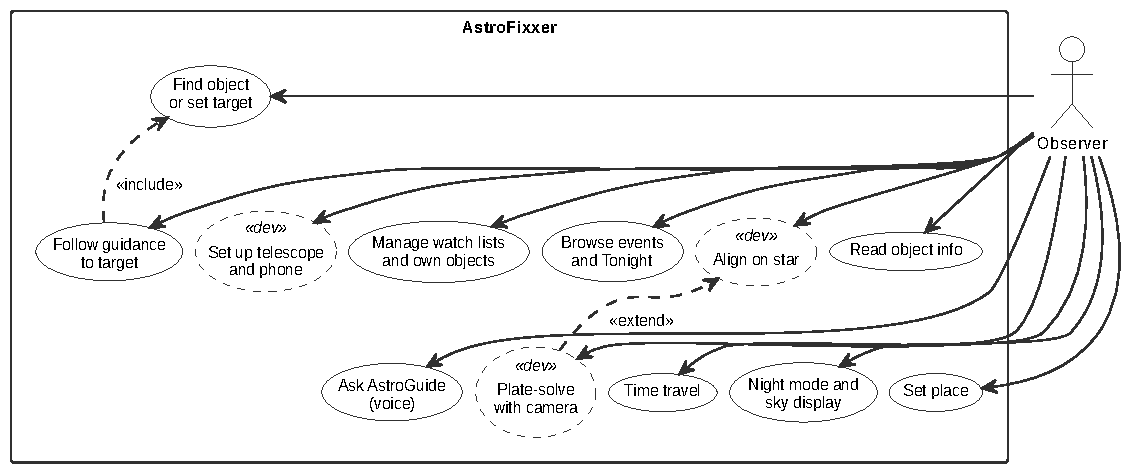
\includegraphics[width=0.9\textwidth]{figures/uml01_usecase.pdf}
\caption{Use cases of the observer. Dashed ovals are in development}
\label{fig:usecase}
\end{figure*}

\subsection{Structure}

Figure~\ref{fig:components} shows the runtime structure. \texttt{MainActivity} is the only code that touches the Android framework. It reads the rotation-vector sensor, gets a location fix, runs speech recognition and speech output, stores settings in shared preferences, loads the assets, and downloads satellite orbit elements from CelesTrak when a network is available. It passes the sensor matrix and settings to \texttt{SkyState} and starts \texttt{SkyScreen}. The \texttt{ui} package has no Android imports and \texttt{astro} does not depend on \texttt{ui}, which is what lets the JVM tests and the desktop harness load each layer alone. \texttt{PlateSolver} and \texttt{SolverStars} are in \texttt{astro} but no screen calls them yet.

\begin{figure*}[tp]
\centering
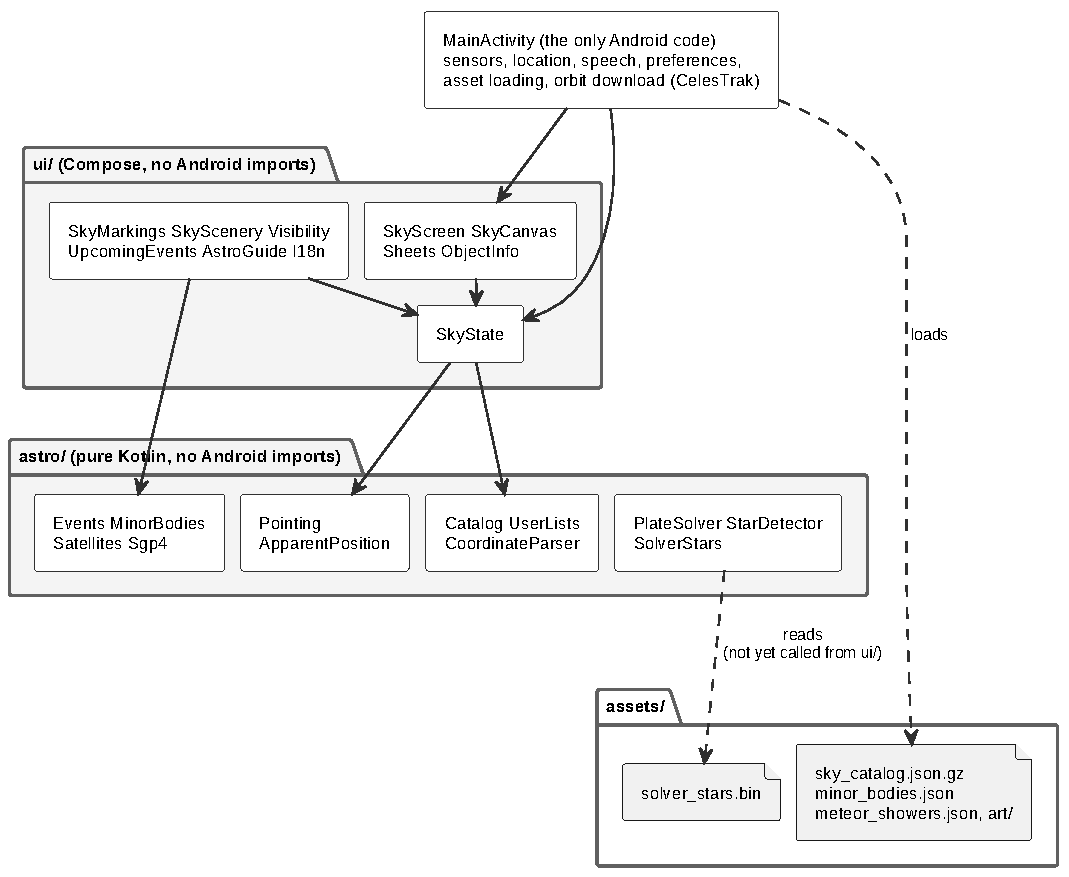
\includegraphics[width=0.8\textwidth]{figures/uml02_components.pdf}
\caption{Components of the app and the assets they read. Dashed arrows are data access}
\label{fig:components}
\end{figure*}

Figure~\ref{fig:classes}(a) gives the core classes. \texttt{SkyState} holds what the screen shows: time, place, phone rotation, pointing mode, alignment state and matrix, the target and the eyepiece settings. Its guidance methods combine the camera frame from \texttt{Pointing} with the ray to the target. \texttt{Catalog} owns the \texttt{SkyObject} list and answers cone, name and constellation queries. The members below the dotted line in \texttt{SkyState}, and \texttt{TelescopeSetup} with its enumerations, exist only in the development branch.


Figure~\ref{fig:classes}(b) shows the solver classes. \texttt{PlateSolver} has two entry points, \texttt{detectStars} and \texttt{solve}. The \texttt{StarSource} interface lets the same solver run on the bright catalogue through \texttt{CatalogStars}, on the 580k-star file through \texttt{SolverStars}, or on a plain list in tests. The result is a sealed class: \texttt{Solved} carries the pose and the false-alarm probability, and \texttt{Failed} carries one of four reasons.

\begin{figure*}[tp]
\centering
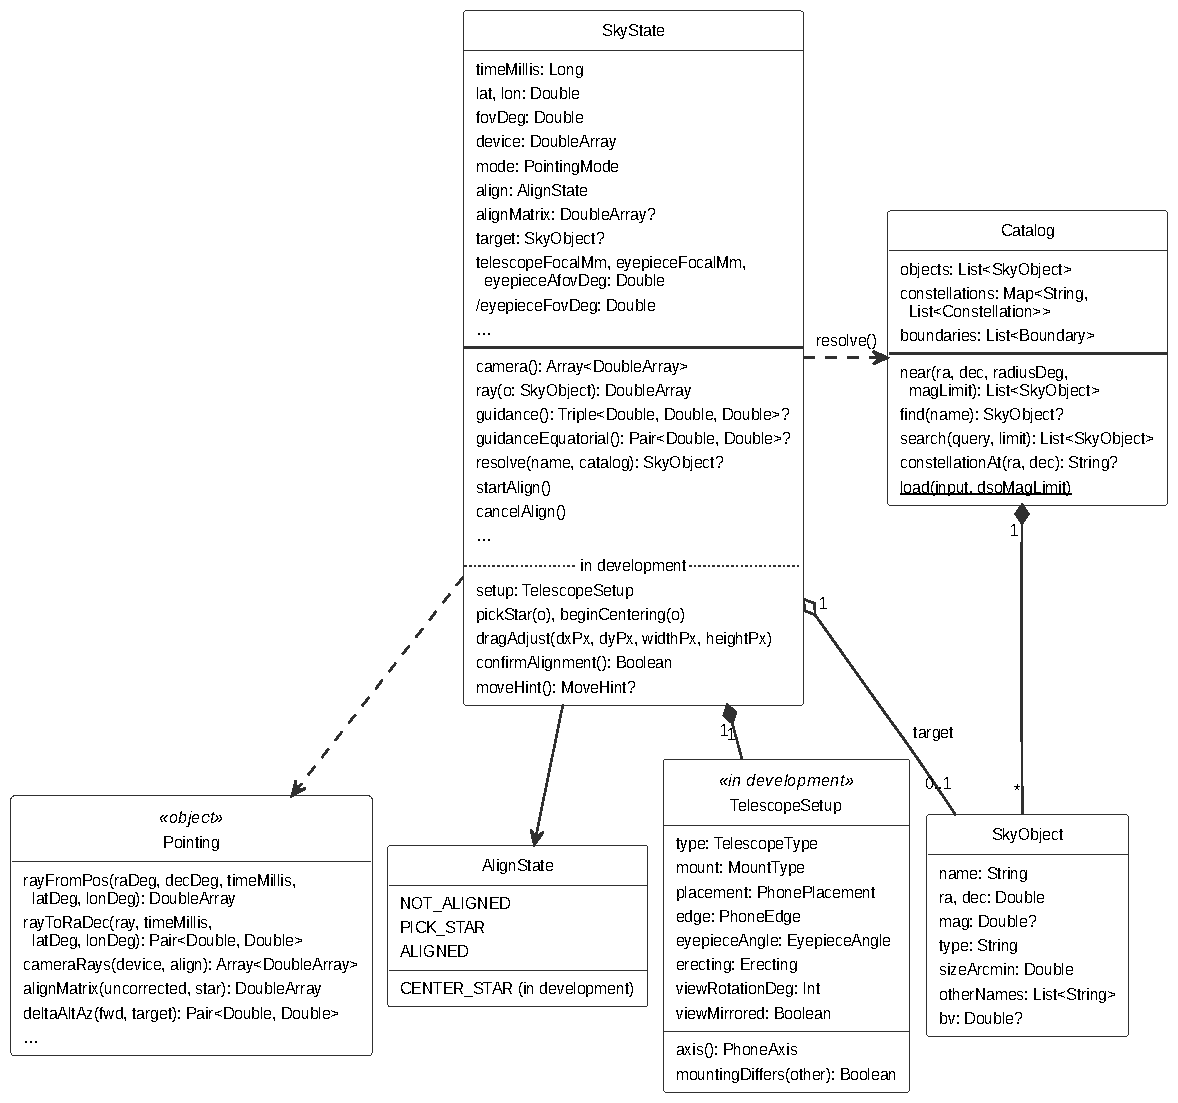
\includegraphics[width=0.72\textwidth]{figures/uml03a_classes_core.pdf}\\[2pt]
(a)\\[6pt]
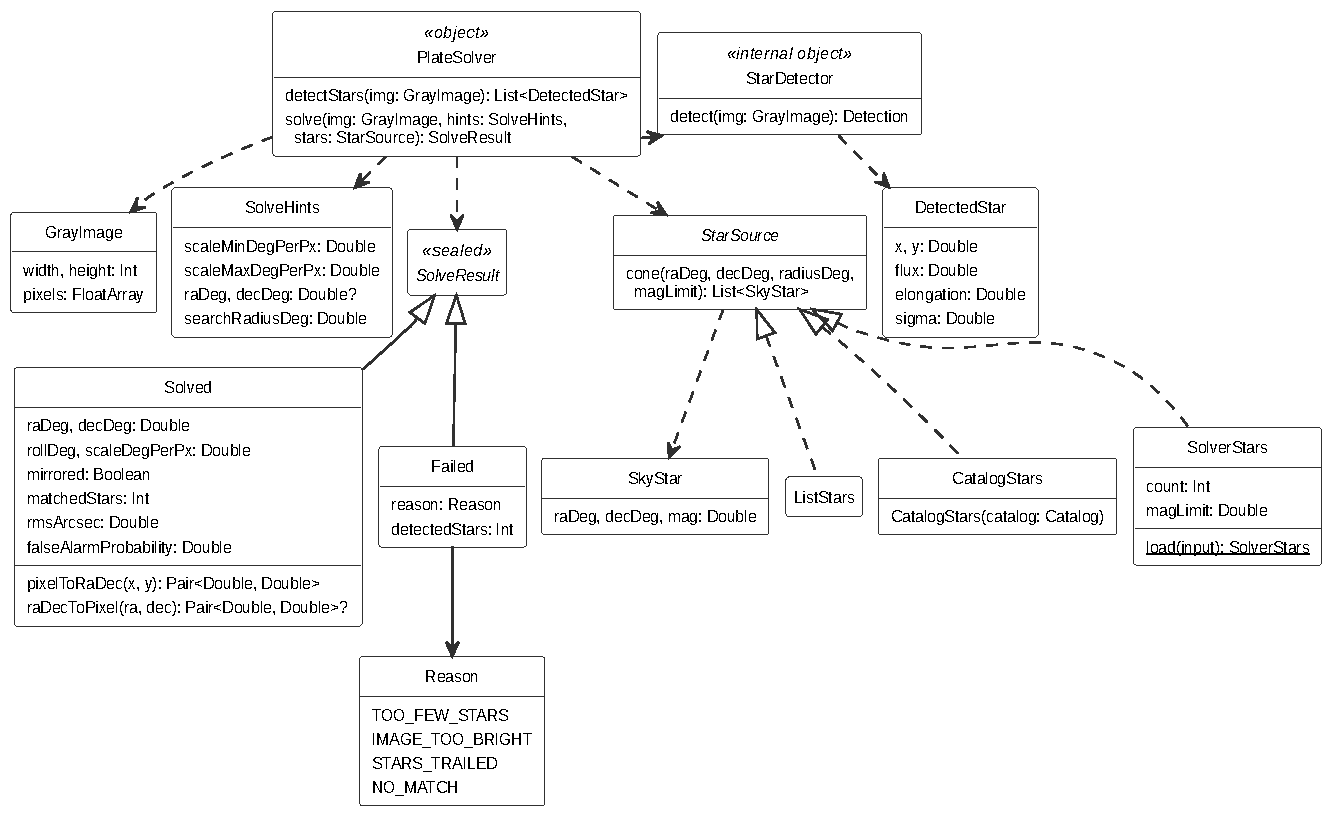
\includegraphics[width=0.76\textwidth]{figures/uml03b_classes_solver.pdf}\\[2pt]
(b)
\caption{Classes of (a) the core model and (b) the plate solver. Members marked in development are not in the released build}
\label{fig:classes}
\end{figure*}

\subsection{Alignment and plate solving}

Figure~\ref{fig:states} shows the alignment states of the revised flow. In the current build, tapping a star while picking aligns at once, as if the telescope were already centred. The revised flow inserts a centring state, so nothing is calibrated until the observer confirms. Cancelling returns to the aligned state if a calibration exists and to the unaligned state otherwise. The calibration is cleared when the phone mounting changes or the settings are reset.

\begin{figure*}[tp]
\centering
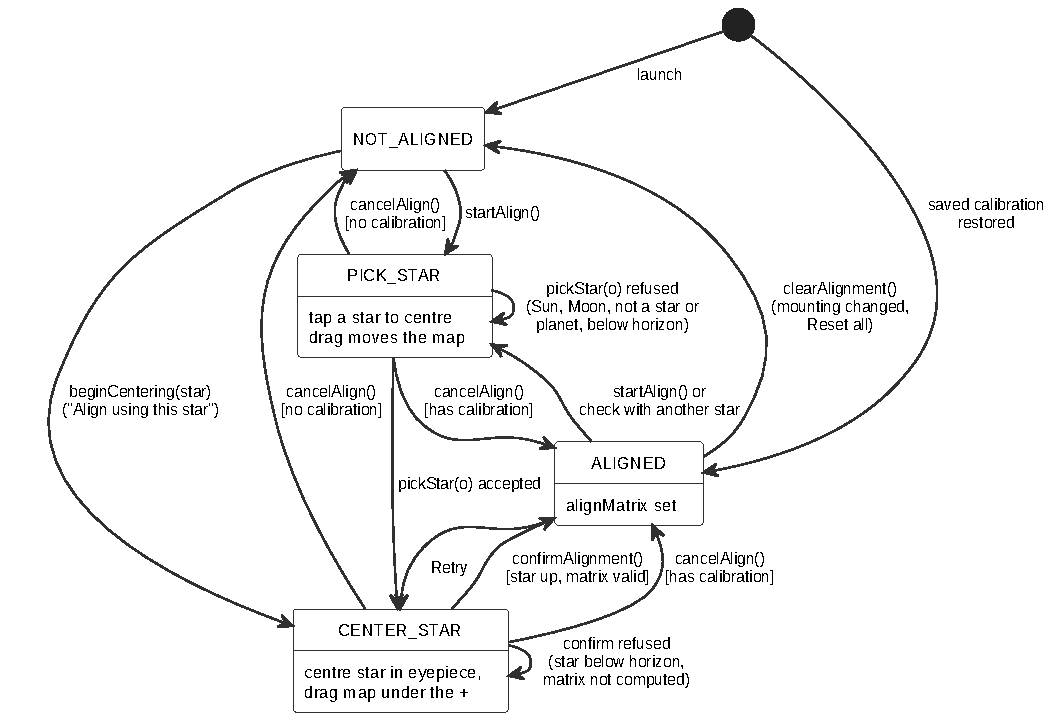
\includegraphics[width=0.7\textwidth]{figures/uml04_states.pdf}
\caption{Alignment states and transitions, from \texttt{SkyState} (in development)}
\label{fig:states}
\end{figure*}

Figure~\ref{fig:sequence} follows one alignment through the classes. The observer starts alignment and taps a star. \texttt{SkyState} accepts it unless it is the Sun, the Moon, not a star or planet, or below the horizon. Dragging the map only changes a pending adjustment, so browsing cannot change the calibration. Confirming computes \texttt{alignMatrix} from the uncorrected camera frame and the star, and rejects it if the corrected axis does not land on the star.

\begin{figure}[tbp]
\centering
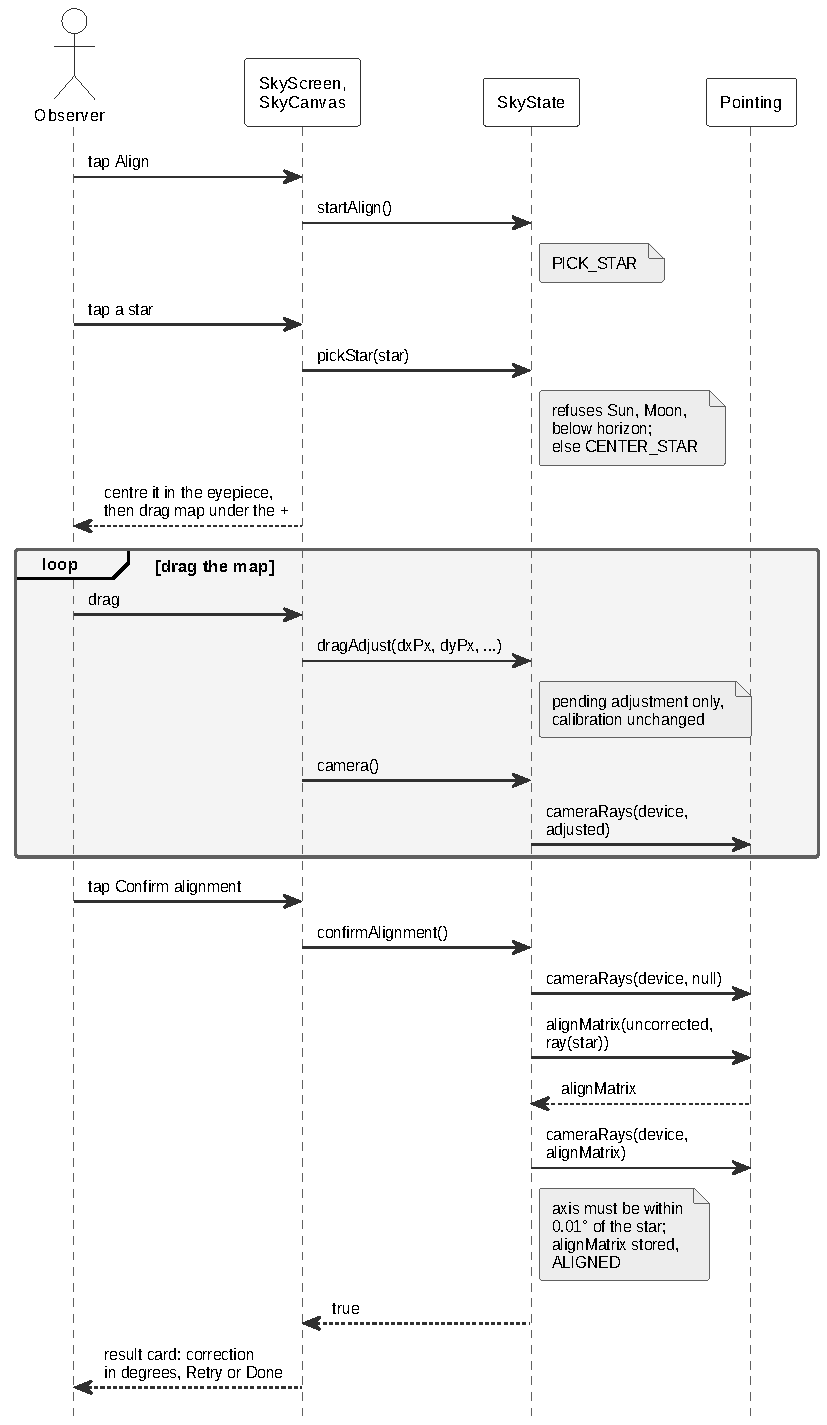
\includegraphics[width=0.9\columnwidth]{figures/uml05_sequence.pdf}
\caption{Star alignment with drag to align (in development)}
\label{fig:sequence}
\end{figure}

Figure~\ref{fig:activity} shows the plate solve as an activity. The three early checks reject a bad image before any matching starts and tell the observer which problem was found. Matching then builds hypotheses from triangles, and each hypothesis is verified against the catalogue. A result is accepted only if it passes the acceptance test described in Section~\ref{sec:solver}; otherwise the solver reports no match.

\begin{figure}[tbp]
\centering
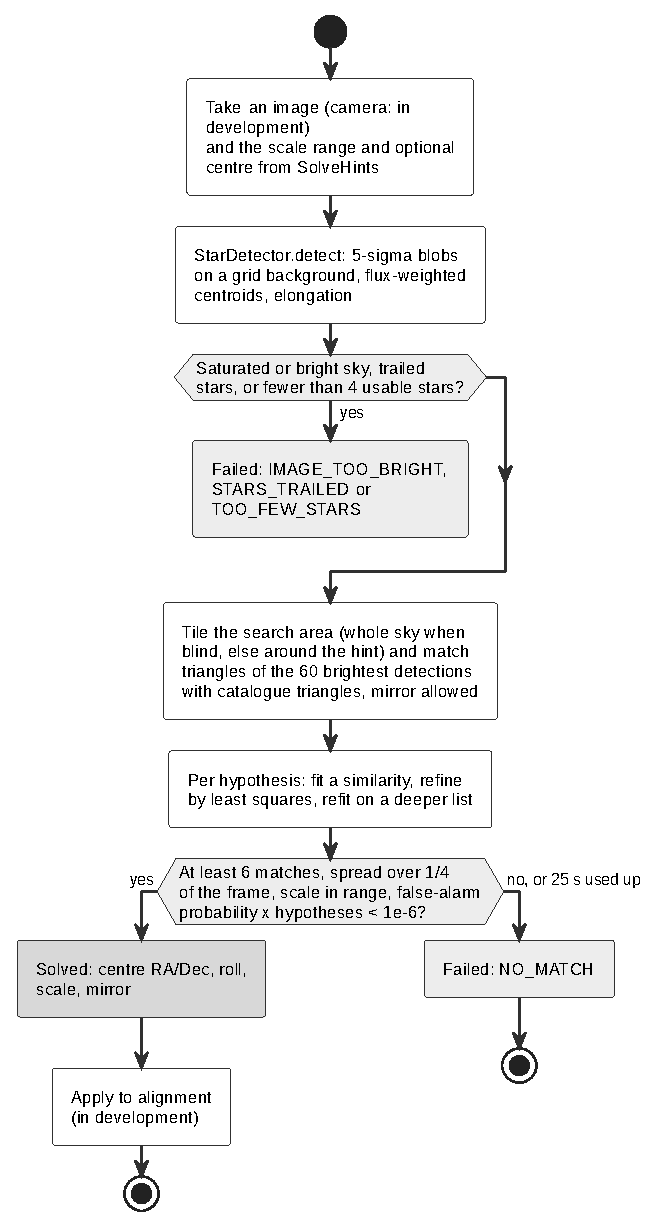
\includegraphics[width=0.8\columnwidth]{figures/uml06_activity.pdf}
\caption{Plate solve, from \texttt{PlateSolver} and \texttt{StarDetector}. Camera capture and applying the result to the alignment are in development}
\label{fig:activity}
\end{figure}

\subsection{Build, test and release}

Figure~\ref{fig:deployment} shows how the code becomes an installed app. The developer runs the importer to write the data assets and pushes the source. Three GitHub Actions jobs run on every push: \texttt{build} runs the JVM tests, assembles the APKs and checks that the sky data is inside the package; \texttt{ui-check} runs the desktop tests and saves screenshots; and \texttt{secret-scan} runs gitleaks over the whole history. A push to the main branch also publishes the latest APK as a GitHub release, and a version tag starts a separate workflow that builds a signed bundle and APK. The phone downloads the APK and needs no network afterwards, except to refresh satellite orbits.

\begin{figure*}[tp]
\centering
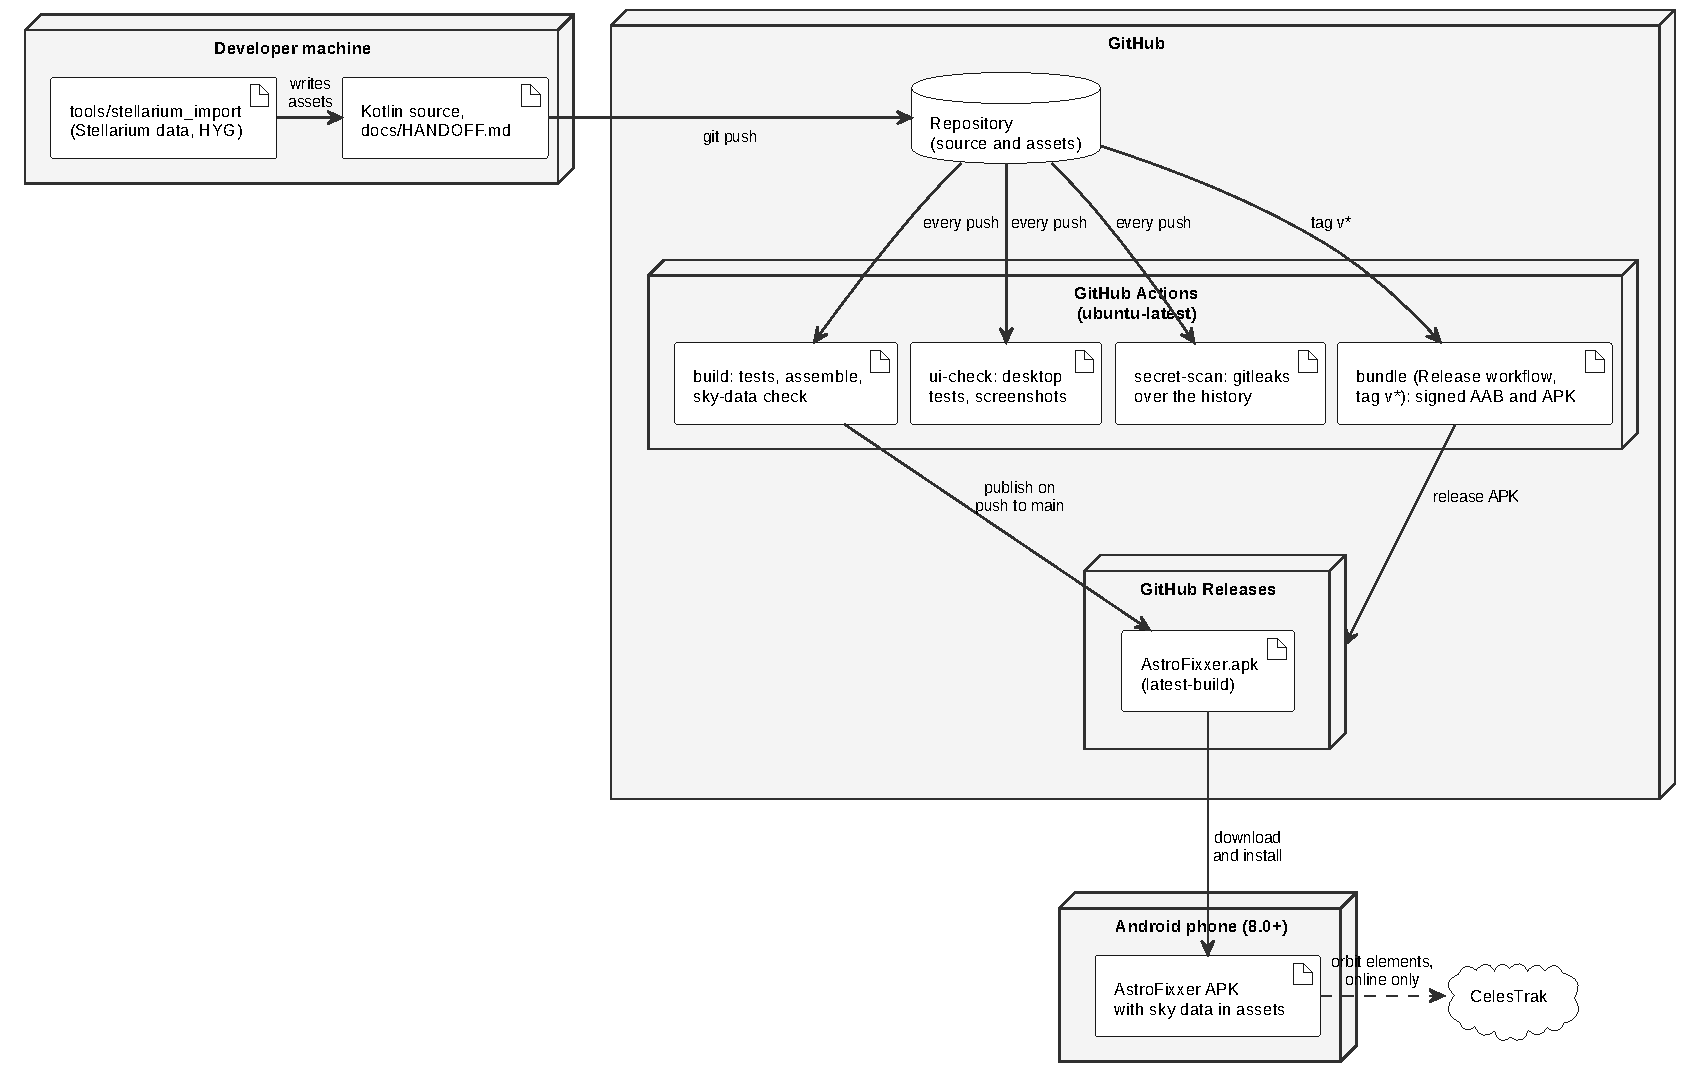
\includegraphics[width=\textwidth]{figures/uml07_deployment.pdf}
\caption{Deployment: from the developer machine through GitHub Actions to the phone}
\label{fig:deployment}
\end{figure*}

\subsection{Development process}

Figure~\ref{fig:process} lists the phases the project followed. Work started from an analysis of the web application and a plan, and the plan went through a review that climbs a ladder of questions (does it need to exist, is it already in the code, does the platform provide it) before any code is written. Each change ends with tests, an entry in the handoff log and a push that starts the CI jobs above. The current phase, 7b, adds the precession fix, the plate solver and the setup and alignment work; the last of these is still open, and the field test is written but has not been run.

\begin{figure}[tbp]
\centering
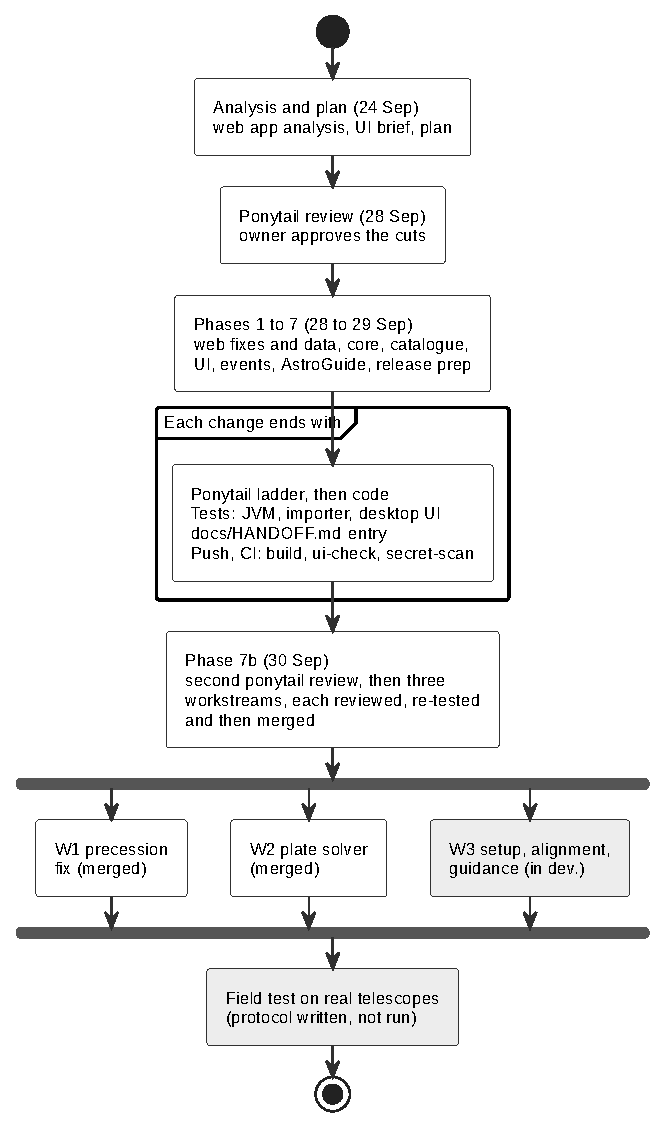
\includegraphics[width=0.75\columnwidth]{figures/uml08_process.pdf}
\caption{Development phases and the steps that end each change}
\label{fig:process}
\end{figure}

\section{Review Against Related Work}
\label{sec:review}

\subsection{Where AstroFixxer differs}

Against AstroHopper and SkEye, AstroFixxer adds a way to measure the pointing instead of trusting the sensors after one alignment. Against StarSense Explorer and PiFinder, it needs no dock, mirror or separate computer; the phone already on the tube does the work. Unlike astrometry.net, the solver does not attempt blind solving at every scale. It uses the scale implied by the observer's equipment and the rough pointing from the sensors, which keeps the star file to 2.94 MB and a hinted solve to about half a second on a desktop CPU. The catalogue is larger than AstroHopper's and is fully offline, which matters at dark sites without mobile coverage. The Indian sky culture and the Hindi interface have no counterpart in the other free tools reviewed here.

\subsection{Limitations and what is not yet tested}

The evidence in Section~\ref{sec:system} comes from unit tests, synthetic images and a desktop test harness. None of it replaces a night at a telescope, and the following points remain open.
\begin{itemize}
\item The plate solver has only seen rendered star fields. Real phone photographs have non-Gaussian star images, compression artefacts, lens distortion beyond the 2\% tested, and noise that depends on the phone's processing. The detection thresholds were tuned on synthetic data.
\item Solving through an eyepiece depends on the phone recording stars of magnitude 9 to 10 in a short exposure. This has not been measured.
\item The revised alignment flow has only run in the desktop test harness, and the camera capture code is still under development. Neither has run on a phone.
\item The coordinate model omits nutation and aberration. At 28 arcseconds this is well inside an eyepiece field, but it would matter for setting-circle readouts on a precisely polar-aligned mount.
\item Sensor drift between alignments has not been measured on real phones or near real tubes.
\end{itemize}
A field protocol is already written: three phones (with and without a magnetometer), two telescopes, and ten Messier objects reached from alignment stars 5 to 20 degrees away, recording the time to target and the misses.

\section{Conclusion}
\label{sec:conclusion}

Free push-to apps put telescope guidance on a phone but cannot check where the telescope points. Camera-based finders can, but only with extra hardware. AstroFixxer brings the two together on an unmodified Android phone: sensor guidance from AstroHopper, an offline Stellarium-derived catalogue, a coordinate model accurate to 28 arcseconds against astropy, and a Kotlin plate solver that found every synthetic test pointing and accepted no false match. The next step is the field test described in Section~\ref{sec:review}, run with real photographs from phones at the eyepiece and beside the tube.

\section*{Acknowledgment}

AstroFixxer is built on the work of others. Artyom Beilis wrote AstroHopper~\cite{astrohopper}, whose pointing code and licence AstroFixxer inherits, and the AstroFixxer web application~\cite{astrofixxerweb} was the starting point for the Android port. All sky data comes from the Stellarium project~\cite{zotti2021}. The solver's star list derives from ESA's Gaia DR3~\cite{gaia2023} and Hipparcos~\cite{perryman1997} catalogues as packaged by Stellarium, and the bright-star catalogue from the HYG database~\cite{hyg}. Greg Miller's public-domain VSOP87 series and CPReduce code supply the planet positions, NASA's Goddard Space Flight Center publishes the eclipse tables, and CelesTrak provides the satellite orbits. Table~\ref{tab:credits} lists every third-party component in the project and its licence.

\begin{table}[h]
\centering
\caption{Third-party repositories, data and libraries}
\label{tab:credits}
\small
\begin{tabular}{@{}p{0.52\columnwidth} p{0.38\columnwidth}@{}}
\toprule
Component & Licence \\
\midrule
AstroHopper / skyhopper (A.~Beilis) & GPLv3 \\
AstroFixxer web app (upstream) & GPLv3 \\
Stellarium deep-sky catalogue, names, meteor showers, minor-body orbits, star catalogues & GPL-2.0-or-later \\
Stellarium sky cultures (modern, Indian) & CC BY-SA 4.0 \\
Stellarium constellation illustrations & Free Art License \\
Gaia DR3 (ESA), via Stellarium & CC BY-SA 3.0 IGO \\
Hipparcos (ESA), via Stellarium & ESA \\
HYG v3 star database & CC BY-SA \\
VSOP87 Java series and CPReduce (G.~Miller) & Public domain \\
NASA eclipse tables (F.~Espenak, NASA GSFC) & Public domain \\
CelesTrak orbital elements & CelesTrak terms \\
Kotlin, Jetpack Compose, AndroidX Activity & Apache 2.0 \\
Compose Multiplatform (desktop test harness) & Apache 2.0 \\
Gradle build tool & Apache 2.0 \\
JUnit 4 & EPL 1.0 \\
Robolectric android-all (compile check) & Apache 2.0 \\
JSON-java (org.json) & See project \\
astropy (reference values only)~\cite{astropy2022} & BSD 3-Clause \\
gitleaks (secret scanning in CI) & MIT \\
\bottomrule
\end{tabular}
\end{table}


\bibliographystyle{IEEEtran}
\bibliography{references}

\end{document}
